\section{\texorpdfstring{Phương pháp nghiên cứu}{methodology}}
% Trình bày chi tiết về ý tưởng, các mô hình toán, các chứng minh nếu có. Đồng thời trình bày các bước thực hiện và khảo sát, kiểm nghiệm kết quả nghiên cứu. Mô tả kết quả nghiên cứu khi thử nghiệm với nhiều tập dữ liệu và những độ khó khác nhau.

\subsection{Ý tưởng thực hiện luận văn}

Nhắc lại yêu cầu bài toán: Tạo sinh video khuôn mặt người đang nói dựa trên một hình ảnh tĩnh chứa mặt người mẫu và một đoạn âm thanh chứa tiếng nói. Qua yêu cầu bài toán ta thấy, đầu vào của hệ thống có tính chất khác với đầu ra, sử dụng hình ảnh tĩnh và âm thanh để tạo ra hình ảnh chuyển động. Một số yêu cầu quan trọng khác quyết định chất lượng của chuỗi hình ảnh được tạo sinh ra cũng cần được chú ý. Đó là:
\begin{itemize}
    \item Hình ảnh phải chân thật, rõ ràng, thể hiện được đúng hình dáng gương mặt người đang nói, không bị méo mó, dị dạng.
    \item Chuỗi hình ảnh được tạo sinh cần phải giữ được đặc trưng gương mặt trong ảnh mẫu. Có nghĩa là, người xem vẫn có thể nhận ra được mặt người đang nói trong video được tạo sinh chính là người trong hình ảnh ban đầu
    \item Khẩu hình miệng khi chuyển động phải khớp với âm thanh được nói ra. Sự chuyển động của môi và miệng trong video được tạo sinh phải thể hiện được cách phát âm từ được nói gần như trong thực tế
\end{itemize}

Dựa theo yêu cầu bài toán, ta cần tìm kiếm một phương pháp để kết hợp đặc trưng âm thanh và hình ảnh lại với nhau, sau đó chuyển đổi đặc trưng này thành video. Để mang lại sự trung thực, sắc nét cho hình ảnh được tạo sinh cũng như lưu giữ được các đặc trưng khuôn mặt người trong hình ảnh ban đầu, chiến thuật của ta là sẽ dựa hoàn toàn trên hình ảnh ban đầu để tạo sinh các khung hình khác trong video. Như vậy, với mỗi khung hình ở mỗi thời điểm $t$ trên video, ta cần phải tìm kiếm sự thay đổi của khung ảnh tại thời điểm đó so với hình ảnh tĩnh được cho ban đầu. Sau đó, ta thực hiện biến đổi hình ảnh được cho ban đầu thành hình ảnh ở khung hình tại thời điểm $t$. Như vậy, câu hỏi đặt ra là ta cần phải thay đổi tại vùng nào trên ảnh mẫu và tại những vùng đó ta sẽ thay đổi như thế nào, thay đổi nhiều hay ít.

Sự thay đổi của hình ảnh được quyết định phần nhiều bởi chuỗi âm thanh được đưa vào hệ thống. Âm thanh giọng nói quyết định khẩu hình miệng và các biểu cảm trên gương mặt. Đôi khi, giọng nói còn có thể quyết định cách chuyển động của đầu. Tuy nhiên, tuy giọng nói góp phần lớn khi định hình sự thay đổi trên gương mặt trong lúc nói, ảnh mẫu ban đầu cũng quyết định phần nào các thay đổi đó. Hình ảnh ban đầu cung cấp thông tin về nhận dạng khuôn mặt, về những đặc điểm của các bộ phận trên gương mặt người nói, về vị trí của mắt, mũi, miệng để định hình cách âm thanh thay đổi hình dạng gương mặt trong lúc nói.

\begin{figure}[H]
    \centering
    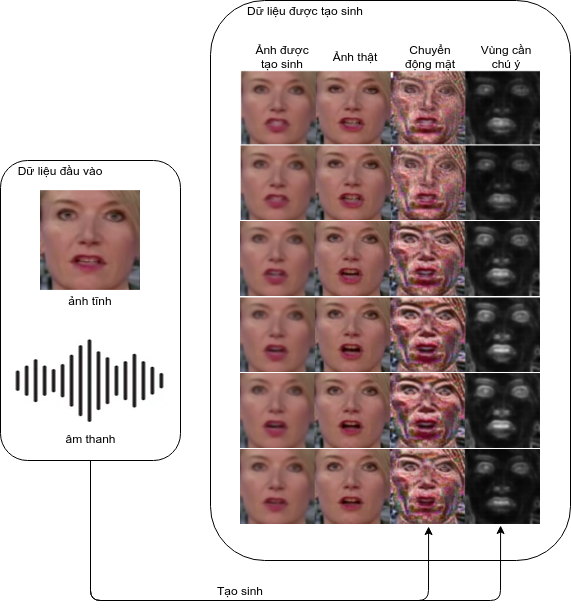
\includegraphics[width=12cm]{./content/materials/idea.png}
    \caption{Ý tưởng về tạo sinh chuỗi hình ảnh chuyển động cho mặt người đang nói}
\end{figure}

Ý tưởng giải quyết bài toán được thể hiện ở hình trên. Chúng ta sẽ tạo ra một hệ thống có khả năng trích xuất đặc trưng của hình ảnh tĩnh ban đầu và âm thanh giọng nói để tạo ra hình ảnh chuyển động của mặt. Tuy nhiên, hình ảnh chuyển động mặt này không hoàn toàn được sử dụng, mà song song với nó, ta tạo ra một mặt nạ tương ứng. Mặt nạ này chỉ chú ý tới một số khu vực trên hình ảnh chuyển động mặt được tạo sinh. Những vùng màu đen là những vùng không được chú ý đến trên ảnh chuyển động vừa được sinh ra, ngược lại, các vùng có màu trắng càng sáng thì càng được chú ý. Như vậy, mặt nạ chú ý sẽ cho ta biết ta nên thay đổi những vùng nào trên gương mặt tại thời điểm $t$ tương ứng với tiếng nói ở thời điểm đó. Đồng thời, hình ảnh chuyển động mặt được tạo sinh song song cho ta biết ta phải thay đổi như thế nào ở những điểm được chú ý. Ở những điểm không được chú ý còn lại, ta sẽ thay thế bằng các điểm ảnh trong ảnh gốc ban đầu. Nhờ vậy, ta có thể bảo toàn được nhận dạng của người nói trong quá trình tạo sinh bằng việc chỉ tìm ra những điểm thay đổi trên gương mặt thay vì cố gắng tìm cách tạo sinh toàn bộ gương mặt của người nói.

\subsection{Mô hình hóa bài toán}

Như phân tích ở phần trên, âm thanh sẽ đóng góp phần lớn vào việc tạo sinh chuyển động cho khuôn mặt. Tuy nhiên, ta thấy dữ liệu dạng sóng biên độ - thời gian của âm thanh dường như không có mối liên hệ tốt với chuyển động trên gương mặt. Vì thế, một bước trích xuất đặc trưng âm thanh để tạo ra một đặc trưng gần gũi hơn với những chuyển động tương ứng trên gương mặt là một bước cần thiết để việc tạo sinh hình ảnh có thể tạo ra những hình ảnh chất lượng tốt và có được những chuyển động chính xác. Do đó, ta sẽ chuyển âm thanh thành một dạng thể hiện khác, đó là các cột mốc trên gương mặt (Facial Landmark). Cột mốc trên mặt gồm 68 điểm trên không gian hai chiều. Mỗi điểm đánh dấu một vị trí trên gương mặt.

\begin{figure}[H]
    \centering
    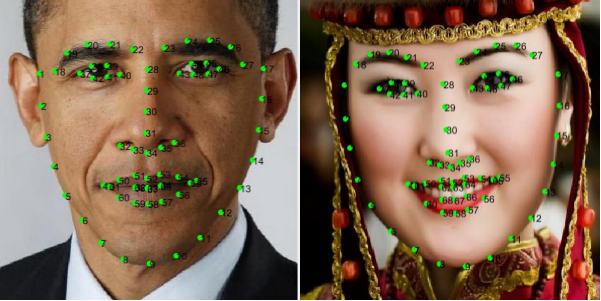
\includegraphics[width=10cm]{./content/materials/landmark_intro.png}
    \caption{Các điểm cột mốc trên khuôn mặt. Hình ảnh được lấy từ bài báo \cite{landmark}}
\end{figure}

Như vậy, từ đoạn âm thanh có chứa tiếng nói và hình ảnh ban đầu, ta sẽ tạo sinh ra một chuỗi cột mốc khuôn mặt để thay thế cho âm thanh làm căn cứ cho những chuyển động trên gương mặt cho phần mạng phía sau. Cấu trúc tổng quát của hệ thống được thế hiện ở Hình \ref{fig:common_architecture}.

\begin{figure}[H]
    \centering
    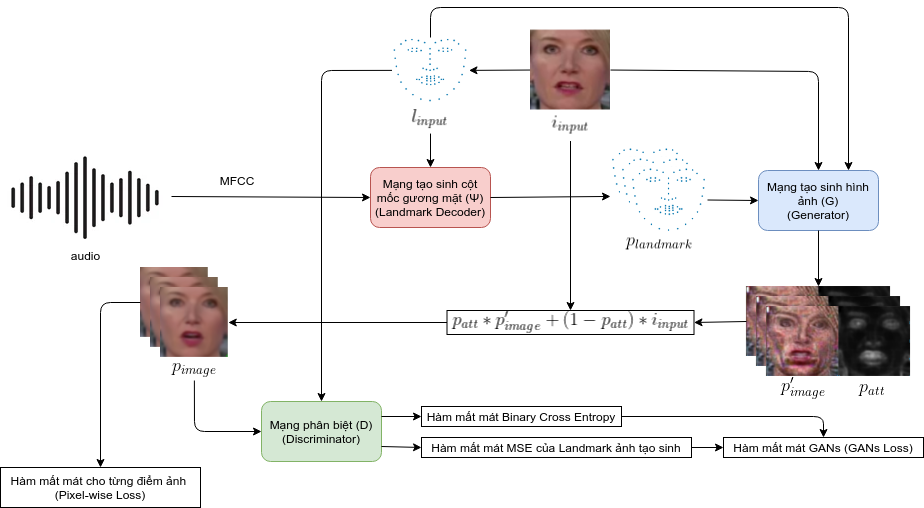
\includegraphics[width=15cm]{./content/materials/common_architecture.png}
    \caption{Cấu trúc tổng quát của hệ thống}
    \label{fig:common_architecture}
\end{figure}

Theo như kiến trúc được thể hiện ở Hình \ref{fig:common_architecture}, hệ thống sẽ trích xuất đặc trưng cột mốc $l_{input}$ trên gương mặt trong hình mẫu $i_{input}$. Sau đó, đặc trưng MFCC sẽ được trích xuất từ âm thanh đầu vào. Đặc trưng MFCC và $l_{input}$ sẽ được đưa vào mạng tạo sinh cột mốc gương mặt (Landmark Decoder). Mạng này kết hợp hai đặc trưng trên với nhau để dự đoán chuỗi các cột mốc gương mặt người khi nói đoạn âm thanh được đưa vào hệ thống ($p_{landmark}$). Từ thời điểm này, âm thanh không còn được sử dụng để tạo sinh hình ảnh mặt người, chuỗi những điểm cột mốc gương mặt $p_{landmark}$ sẽ thay thế cho đặc trưng âm thanh trong những bước xử lý tiếp theo. Như vậy, ta đã tách rời được dữ liệu âm thanh so với phần tạo sinh hình ảnh, và cung cấp cho phần mạng phía sau thông tin dễ học hơn, giàu thông tin hữu ích hơn và ít nhiễu hơn. 

Phần tiếp theo trong hệ thống là cặp mạng tạo sinh (Generator) và phân biệt (Discriminator) tạo nên mạng GANs như đã trình bày ở phần \ref{sec:base_knowledge_gans}. Tuy nhiên, đây không phải là mạng GANs truyền thống mà là mạng GANs có điều kiện (Conditional GANs). Thay vì tạo sinh dữ liệu bằng một véc tơ được sinh ra ngẫu nhiên theo phân phối chuẩn, mạng GANs có điều kiện dựa vào một điều kiện đầu để tạo sinh dữ liệu. Trong luận văn này, mạng GANs có điều kiện tạo sinh dữ liệu với điều kiện đầu vào là $i_{input}$, $l_{input}$ và $p_{landmark}$.

Bài toán mà mạng tạo sinh phải giải là đối với mỗi khung ảnh được tạo sinh để phù hợp với giọng nói được cho, ta phải thay đổi hình ảnh gốc $i_{input}$ ở những vị trí nào, và tại vị trí đó, ta phải thay đỏi nó như thế nào để sinh ra được hình ảnh mới? Mạng tạo sinh hình ảnh với đầu vào là hình ảnh mẫu $i_{input}$, cột mốc của gương mặt của hình ảnh mẫu $l_{input}$ và chuỗi cột mốc gương mặt vừa được tạo sinh $p_{landmark}$ có chức năng tạo sinh ra hai chuỗi dữ liệu $p_{att}$ và $p'_{image}$ tương ứng để trả lời cho câu hỏi trên. Chuỗi hình ảnh $p_{att}$ và $p'_{image}$ có cùng chiểu dài và kích thước hình ảnh. Chuỗi hình ảnh $p_{att}$ thể hiện những điểm cần thay đổi trên ảnh gốc và mức độ thay đổi tại điểm đó. Chuỗi dữ liệu còn lại là chuỗi $p'_{image}$ thể hiện những thay đổi trên ảnh gốc để phù hợp với tiếng nói trong âm thanh. Chuỗi $p'_{image}$ có cấu trúc hình ảnh là gương mặt người, có sự thay đổi theo trục thời gian tương ứng với những chuyển động trên gương mặt để phù hợp với giọng nói. Tuy nhiên đây không phải là hình ảnh hoàn chỉnh của gương mặt, chỉ một vài chi tiết cần thiết trên chuỗi $p'_{image}$ được lấy ra và ghép vào ảnh gốc $i_{input}$ để tạo ra hình ảnh cuối cùng. Cũng vì vậy, $p'_{image}$ là chuỗi hình ảnh được sinh ra để cho ta biết hình ảnh gốc nên thay đổi như thế nào. 

Cuối cùng, ta cần phải kết hợp hình ảnh ban đầu $i_{image}$ và chuỗi hình ảnh vừa được sinh ra là $p'_{image}$ và $p_{att}$ lại để tạo thành chuỗi hình ảnh hoàn chỉnh $p_{image}$. Có thể gọi $p_{att}$ là một mặt nạ chú ý (attention map), mặt nạ này có giá trị các điểm ảnh trong khoảng từ 0 đến 1. Với điểm ảnh càng gần về 0, điểm ảnh cùng vị trí trong $i_{input}$ càng được sử dụng nhiều, điểm ảnh cùng vị trí trong $p'_{image}$ càng ít được sử dụng. Và ngược lại, nếu điểm ảnh trong $p_{att}$ càng gần về 1, điểm ảnh cùng vị trí trong $i_{input}$ càng ít được sử dụng, điểm ảnh cùng vị trí trong $p'_{image}$ càng được sử dụng nhiều. Công thức tạo thành $p_{image}$ được biểu diễn như sau:

\begin{equation}
    p_{image}=p_{att}*p'_{image}+(1-p_{att})*i_{input}
\end{equation}

Hình ảnh hoàn chỉnh được tạo sinh $p_{image}$ sau đó được đem đi so sánh với chuỗi hình ảnh trong video gốc để tính giá trị mất mát L1 cho chuỗi hình ảnh tạo sinh. Giá trị mất mát này được lan truyền ngược để cập nhật các trọng số trong mạng tạo sinh. Chuỗi hình ảnh hoàn chỉnh cũng được đưa vào bộ phân biệt (Discriminator) để bộ phân biệt dự đoán xem chuỗi hình ảnh này là ảnh được tạo sinh (chuỗi hình ảnh giả) hay chuỗi hình ảnh này là hình ảnh được lấy từ tập dữ liệu thật, sai sót của bộ phân biệt được biểu diễn bằng hàm Binary Cross Entropy. Đồng thời bộ phân biệt cũng dựa vào chuỗi hình ảnh được đưa vào và cột mốc gương mặt của ảnh mẫu $l_{input}$ để cố gắng sinh ra một chuỗi cột mốc gương mặt tương ứng với chuỗi hình ảnh $p_{image}$ được đưa vào mạng. Chuỗi cột mốc gương mặt vừa được sinh ra này sẽ được so sánh với chuỗi cột mốc gương mặt được rút trích trực tiếp từ chuỗi hình ảnh trong video gốc. Sự sai khác trong hai chuỗi cột mốc gương mặt được tính bằng hàm mất mát MSE. Điều này có nghĩa, chuỗi hình ảnh được tạo sinh $p_{image}$ phải rút trích được một chuỗi cột mốc gương mặt sao cho giống nhất với chuỗi cột mốc gương mặt trong video gốc. Tổng hợp của giá trị mất mát MSE và Binary Cross Entropy vừa nêu, ta được hàm mất mát GANs chung của mạng GANs. Giá trị mất mát GANs này được lan truyền ngược để cập nhật trọng số cho cả mạng tạo sinh và mạng phân biệt.

\subsection{Các tập dữ liệu được sử dụng}
\subsubsection{Tập dữ liệu GRID \cite{grid}}

Tập dữ liệu GRID là tập dữ liệu được tạo ra từ phòng nghiên cứu của Đại học Sheffield tại Anh. Tập dữ liệu này được tạo ra để hỗ trợ cho việc phân tích và nghiên cứu gương mặt người khi nói, bao gồm các nghiên cứu về nhận thức gương mặt thông qua giọng nói và nhận diện giọng nói. Tập dữ liệu chứa 1000 câu, được nói bởi 34 người khác nhau. Như vậy, tập dữ liệu này chứa 34000 video với chất lượng cao, mỗi video có độ dài 3 giây. Những câu được nói rất đơn giản, với cú pháp: <động từ (4 từ)> <màu sắc (4 từ)> <giới từ (4 từ)> <chữ cái (25 chữ)> <số (10 số)> <trạng từ (4 từ)>. Các cụm từ giống hệt nhau về mặt cú pháp đã nêu ở trên (ví dụ như câu "place green at B 4 now"), được phát âm rõ và đọc với tốc độ bình thường, âm thanh được thu ở môi trường kín, không nhiễu. Hình ảnh trong video rõ nét, được quay với phông nền xanh với điều kiện ánh sáng tốt. Mặt người khi nói ít chuyển động (ít xoay, ít lắc đầu) và được quay trực diện. Gương mặt người khi nói không biểu lộ cảm xúc và người nói chớp mắt một cách tự nhiên. Tập dữ liệu GRID được chia làm hai tập huấn luyện và kiểm thử. Video được chia thành 3 tập huấn luyện, tập kiểm chứng và tập kiểm thử với tỉ lệ 90\%-5\%-5\% tương ứng.

\begin{figure}[H]
    \centering
    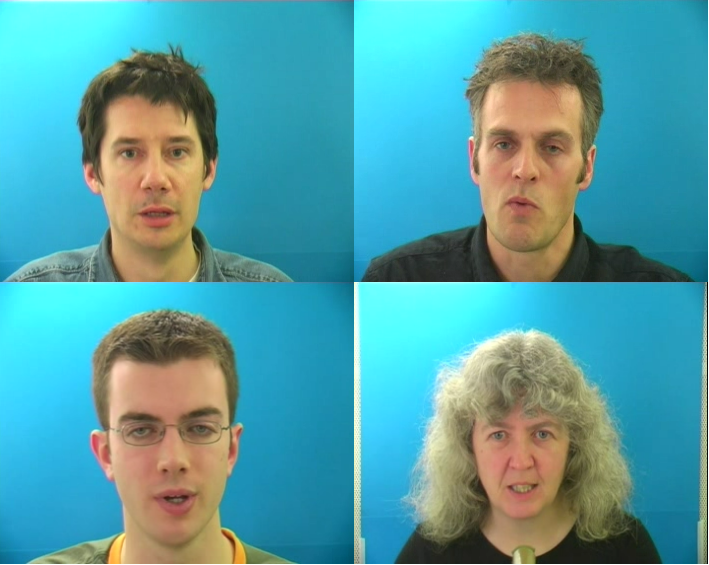
\includegraphics[width=12cm]{./content/materials/grid.png}
    \caption{Ảnh trích xuất từ các video trong tập dữ liệu GRID}
\end{figure}

\subsubsection{Tập dữ liệu LRW \cite{lrw}}

Tập dữ liệu LRW là tập dữ liệu được xây dựng bởi một nhóm nghiên cứu từ trường Đại học Oxford và sở hữu bởi hãng tin tức BBC. Đây là tập dữ liệu lớn, với những đoạn video ngắn được cắt từ những đoạn video được phát trên kênh BBC. Khác với tập dữ liệu GRID, video trong tập LRW là những video được thu trong môi trường tự nhiên. Tập dữ liệu LRW có hơn 1 triệu video khác nhau, mỗi video có độ dài 1.16 giây, gồm 29 khung hình. Những video này được chia làm 1000 từ vựng, mỗi từ vựng được nói bởi hơn 1000 người khác nhau. Tổng cộng, tập dữ liệu LRW chứa gần 1000 giờ video. Tuy nhiên, do video được cắt ghép từ video được thu trong môi trường tự nhiên, tín hiệu trong video có độ nhiễu nhất định. Âm thanh trong video có thể nghe rõ lời nói, tuy nhiên một số lượng không nhỏ video bị lẫn tiếng ồn và các tạp âm khác. Về mặt hình ảnh, video có hình ảnh rõ nét, lấy điểm trên đầu mũi của người đang nói làm trung tâm, vì vậy, với các video mà người nói có sự cử động ở đầu như xoay hay lắc đầu, video sẽ bị rung lắc mạnh để giữ điểm đầu mũi ở giữa khung hình. Mặt người trong video được quay ở nhiều vị trí khác nhau và có thể lệch về một phía (quay từ phía bên trái, bên phải, hoặc lệch theo chiều dọc gương mặt). Với mỗi từ ngữ, tập dữ liệu đã chia sẵn thành 3 tập tập huấn luyện, tập kiểm chứng và tập kiểm thử với số lượng video tương ứng cho mỗi loại là 1000-50-50.

\begin{figure}[H]
    \centering
    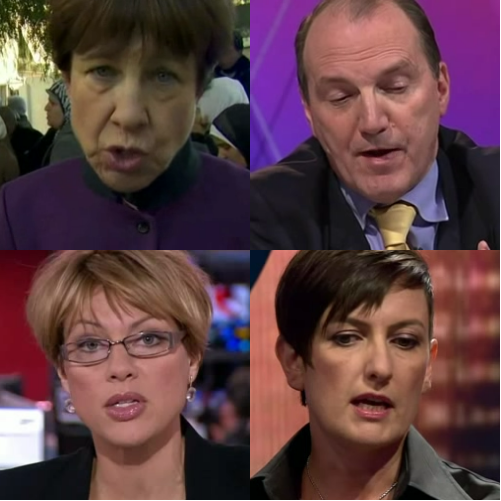
\includegraphics[width=12cm]{./content/materials/lrw.png}
    \caption{Ảnh trích xuất từ các video trong tập dữ liệu LRW}
\end{figure}

\subsection{Tiền xử lý dữ liệu}

\subsubsection{Tiền xử lý âm thanh}
Ta có thể thấy, phần âm thanh ta chú ý đến chỉ là tiếng nói của con người và muốn loại bỏ các tạp âm. Tần số âm thanh của giọng nói con người dao động trong khoảng từ 20Hz đến 20kHz, và theo như phương pháp lấy mẫu Nyquist, để lấy mẫu một tín hiệu có tần số $x$(Hz), thì bộ lấy mẫu phải lấy mẫu ở tần số ít nhất là $2x$(Hz). Như vậy, khi thu âm, để thu được âm thanh mà con người có thể nghe được, người ta phải lấy mẫu ở tần số thấp nhất là 40kHz. Trên thực tế, trong việc ghi âm, người ta thường lấy mẫu ở tần số 44.1kHz. Đây đã trở thành tiêu chuẩn chung, hầu hết các video có âm thanh thì âm thanh trong video phần lớn được lấy mẫu ở tần số này. Âm thanh trong tập dữ liệu GRID và LRW cũng được lấy mẫu ở tần số 44.1kHz.

\begin{figure}[H]
    \centering
    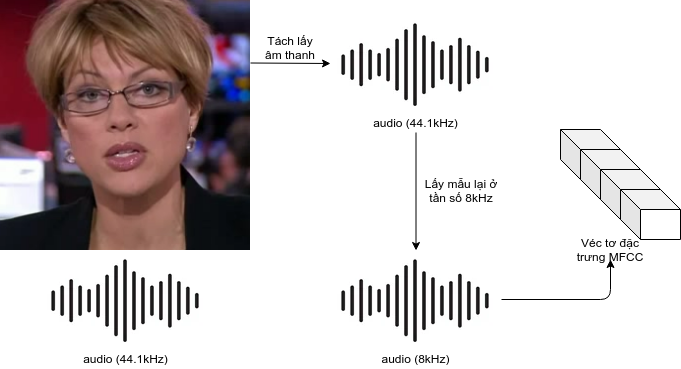
\includegraphics[width=12cm]{./content/materials/preprocess-audio.png}
    \caption{Tiền xử lý tín hiệu âm thanh}
\end{figure}

Tuy nhiên, thanh quản con người chỉ có thể phát ra âm thanh với tần số dưới 4kHz. Vì vậy, để loại bỏ nhiễu ở các dãi tần số cai hơn, ta có thể lấy mẫu lại âm thanh trong video. Theo phương pháp lấy mẫu Nyquist, để lấy được âm thanh có tần số dưới 4kHz, ta cần phải lấy mẫu ở tần số 8kHz. Như vậy, tất cả âm thanh trong tất cả các đoạn video sẽ được lấy mẫu lại ở tần số 8kHz. Bộ lấy mẫu sẽ hoạt động như một bộ lọc thông thấp để loại bỏ nhiễu cao tần trong các đoạn âm thanh. Phương pháp lấy mẫu tần số thấp này cũng được dùng trong các thiết bị thu tiếng nói như máy thu âm, điện thoại để loại bỏ nhiễu.

Âm thanh sau khi lấy mẫu lại sẽ được đem đi trích xuất để lấy đặc trưng MFCC. Như đã nói ở phần \ref{sec:base_knowledge_mfcc}, MFCC là đặc trưng âm thanh chỉ dành riêng cho tiếng nói của con người. Ta tiến hành lấy đặc trưng MFCC với của sổ trượt 10ms, cứ mỗi cửa sổ trượt 10ms sẽ sinh ra một véc tơ 13 chiều tương ứng với 13 quãng tần số khác nhau, tuy nhiên ta chỉ sử dụng 12 khoảng tần số đầu và loại bỏ khoảng cuối. Như vậy, với thời lượng 3 giây, âm thanh trong tập LRW sẽ sinh ra một ma trận đặc trưng MFCC có kích thước 12x300, tương tự là kích thước ma trận MFCC 12x116 của các đoạn âm thanh trong tập dữ liệu LRW.

\subsubsection{Tiền xử lý hình ảnh và trích xuất cột mốc gương mặt}

Đầu tiên, tất cả các khung hình của tất cả các video sẽ được nhận diện khuôn mặt bằng mô hình nhận diện khuôn mặt của thư viện Dlib. Từ khung hình đã được nhận diện khuôn mặt này, ta dễ dàng tìm được cột mốc gương mặt trên từng khung hình. Đầu tiên, ta cần tìm ra một cốt mốc gương mặt được dụng để làm chuẩn nhằm chuẩn hóa cho tất cả những cột mốc gương mặt còn lại. Cột mốc gương mặt chuẩn là cột mốc gương mặt có hình dáng chung chung của mặt người, và không có chứa đặc điểm riêng của gương mặt của bất kì người nào. Như vậy, để tìm ra cột mốc gương mặt chuẩn, ta cần tính giá trị trung bình của một số lượng lớn các cột mốc gương mặt trong các tập dữ liệu hiện có. Do tập dữ liệu LRW có độ nhiễu cao, nên ta sẽ sử dụng tập dữ liệu GRID để tính cột mốc gương mặt chuẩn. Đầu tiên, ta tính giá trị trung bình của tất cả các cột mốc gương mặt trên tất cả các khung hình của tập GRID. Sau đó, ta dùng phép biến đổi tuyến tính trên không gian hai chiều (Affine Transformation) để đưa hai điểm ở vùng ngoài của mắt (điểm 37 và 46 trên hình \ref{fig:standard_landmark}) về tọa độ $(0.3, 0.33)$ và $(0.7, 0.33)$ tương ứng.

\begin{figure}[H]
    \centering
    \subfloat[Cột mốc gương mặt đánh số]{{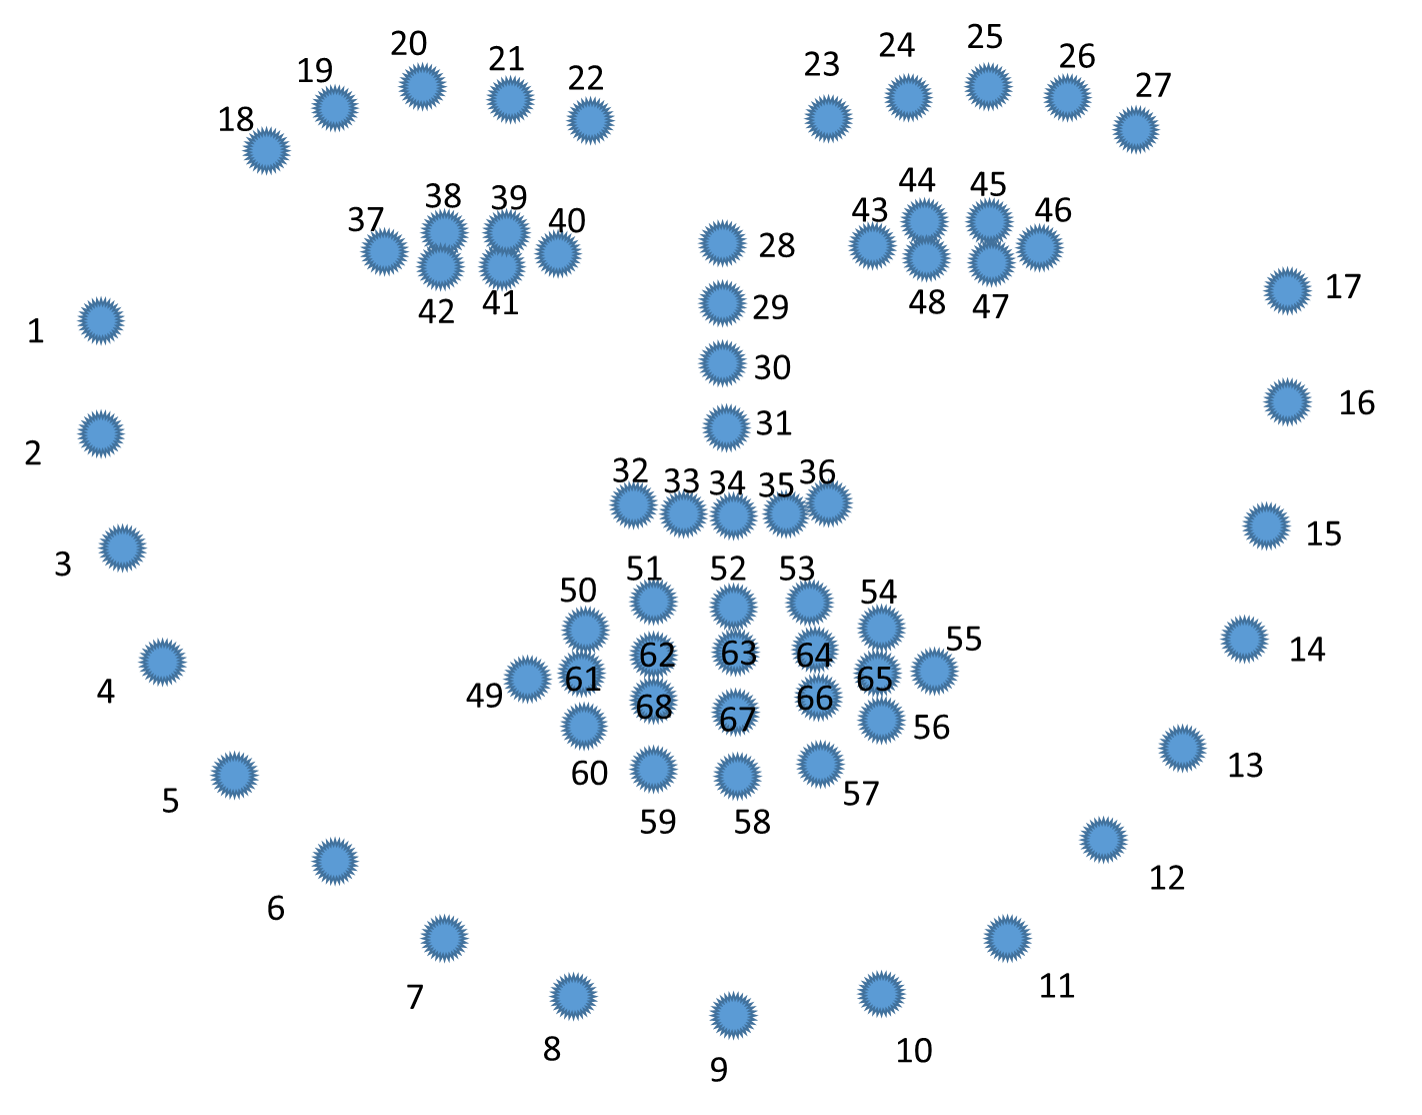
\includegraphics[width=7cm]{./content/materials/enum_landmark.png} }}
    \qquad
    \subfloat[Cột mốc gương mặt được dùng làm chuẩn]{{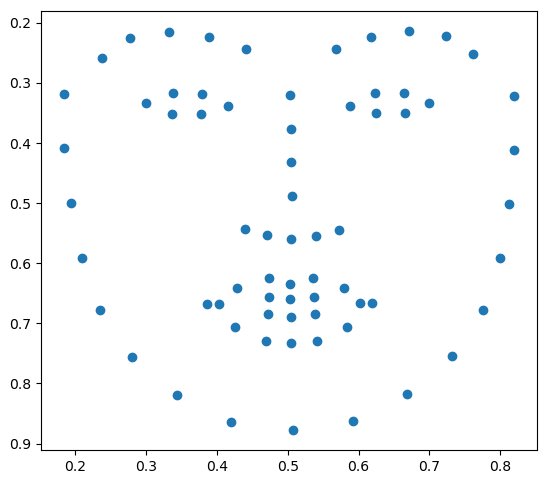
\includegraphics[width=7cm]{./content/materials/standard_landmark.png} }}
    \caption{Xử lý cột mốc gương mặt}
    \label{fig:standard_landmark}
\end{figure}


\subsection{Cấu trúc chi tiết của hệ thống}

\subsubsection{Cấu trúc của bộ giải mã landmark của khuôn mặt (Landmark Decoder)}

\begin{figure}[H]
    \centering
    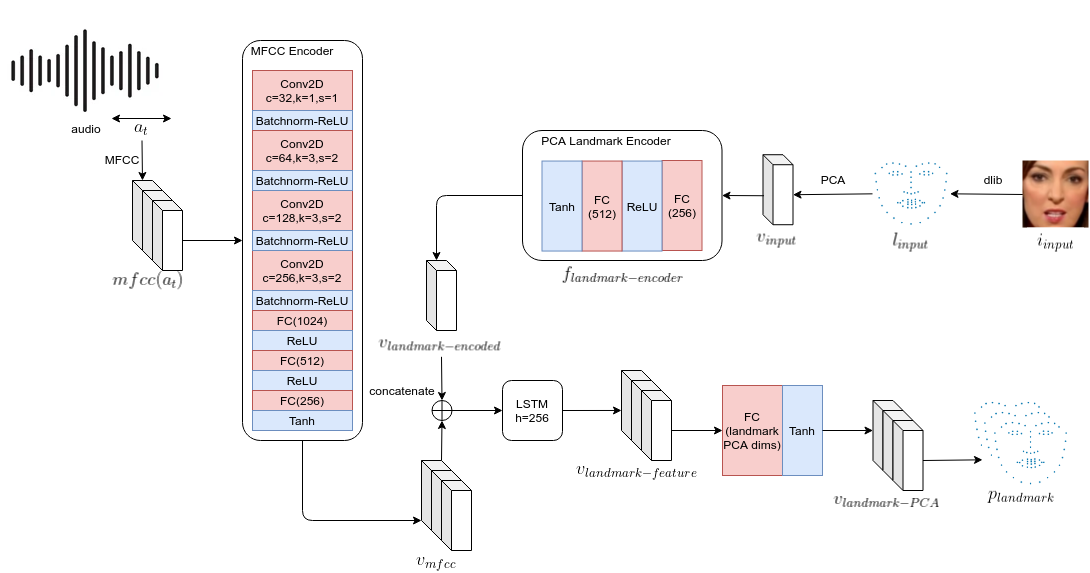
\includegraphics[width=15cm]{./content/materials/landmark_decoder.png}
    \caption{Cấu trúc của bộ giải mã landmark của khuôn mặt (Landmark Decoder)}
\end{figure}



\subsubsection{Cấu trúc của bộ tạo sinh hình ảnh (Generator)}

\begin{figure}[H]
    \centering
    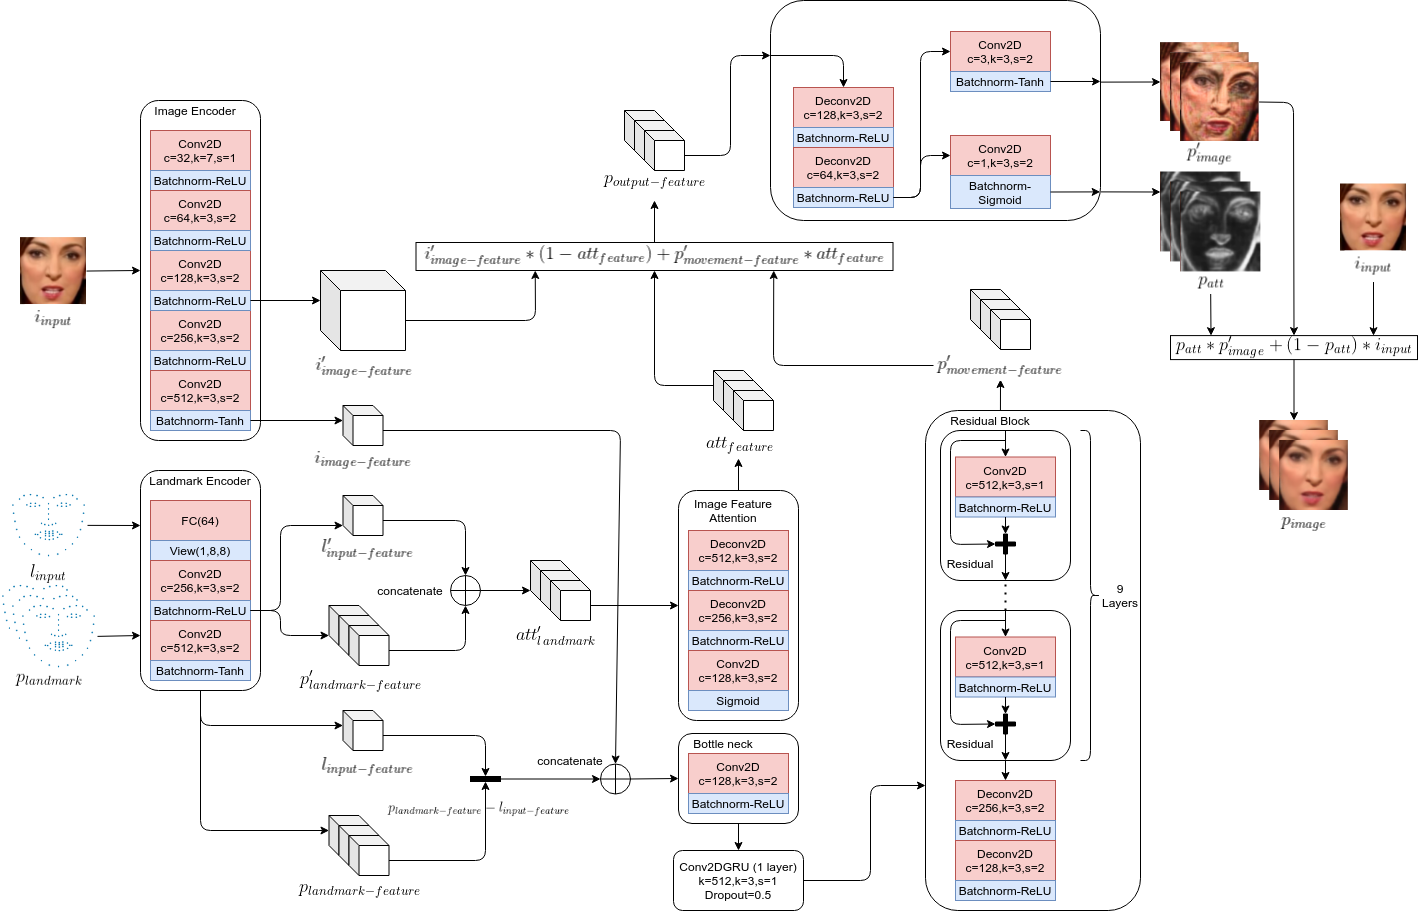
\includegraphics[width=15cm]{./content/materials/generator.png}
    \caption{Cấu trúc của bộ giải mã landmark của khuôn mặt (Generator)}
\end{figure}

\subsubsection{Cấu trúc của bộ phân biệt hình ảnh (Discriminator)}

\begin{figure}[H]
    \centering
    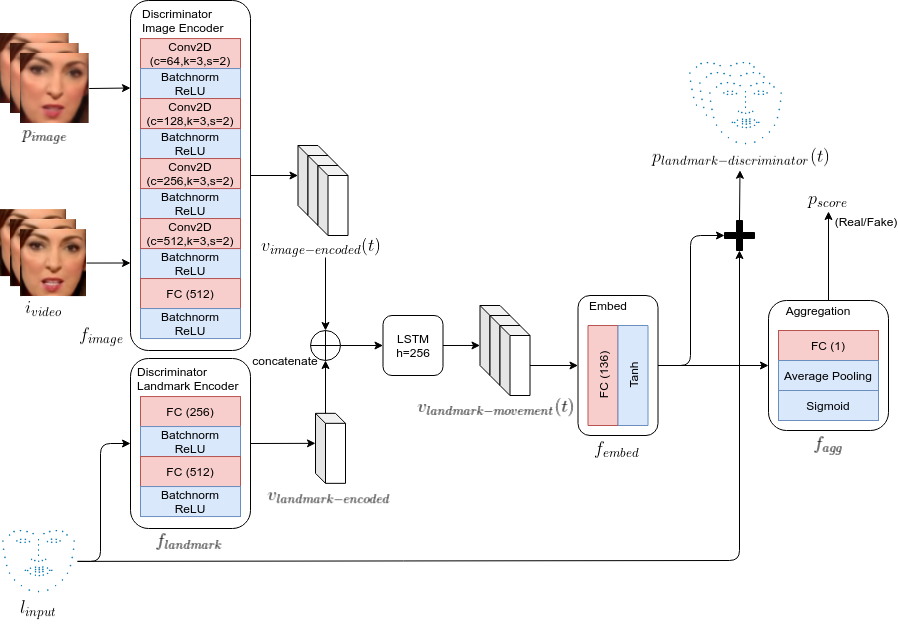
\includegraphics[width=15cm]{./content/materials/discriminator.png}
    \caption{Cấu trúc của bộ phân biệt hình ảnh (Discriminator)}
\end{figure}

\subsubsection{Hàm mất mát được sử dụng cho hệ Generator - Discriminator}
